\documentclass[12pt,a4paper]{article}
\usepackage[T5]{fontenc}
\usepackage[utf8]{inputenc}
\usepackage[vietnamese]{babel}
\usepackage{mathptmx} % Font Times New Roman chuẩn
\usepackage{anyfontsize} % Hỗ trợ exact font size 15pt, 18pt
\usepackage{amsmath}
\usepackage{amsfonts}
\usepackage{amssymb}
\usepackage{graphicx}
\usepackage{geometry}
\usepackage{float}
\usepackage{booktabs}
\usepackage{array}
\usepackage{multirow}
\usepackage{hyperref}
\usepackage{listings}
\usepackage{listingsutf8}
\usepackage{xcolor}
\usepackage{caption}
\usepackage{subcaption}
\usepackage{enumitem}
\usepackage{longtable} 
\usepackage{mdframed}
\usepackage{lastpage}
\usepackage{fancyhdr}
\usepackage{pdfpages} % Hỗ trợ chèn file PDF D2, D3
\usepackage{tikz}
\usetikzlibrary{calc}

\geometry{top=2.5cm, bottom=2.5cm, left=3cm, right=2cm}

% Code listing style
\lstset{
    language=Python,
    basicstyle=\ttfamily\footnotesize,
    commentstyle=\color{gray},
    keywordstyle=\color{blue},
    numberstyle=\tiny\color{gray},
    stringstyle=\color{red},
    breaklines=true,
    frame=single,
    showstringspaces=false
}

\hypersetup{
    colorlinks=true,
    linkcolor=black,
    filecolor=blue,      
    urlcolor=blue,
    citecolor=black
}

%%% Custom section numbering & TOC depth
\setcounter{secnumdepth}{4}
\setcounter{tocdepth}{3}

%%% Header & Footer setup
\setlength{\headheight}{45pt}
\pagestyle{fancy}
\fancyhead{} % clear all header fields
\fancyhead[L]{%
  \begin{tabular}{rl}
    
\includegraphics[width=10mm]{IMAGE/LOGO HCMUT.png} &
    \parbox[b]{13cm}{%
      \textbf{TRƯỜNG ĐẠI HỌC BÁCH KHOA - ĐHQG-HCM}\\[1pt]
      \textbf{KHOA KHOA HỌC VÀ KỸ THUẬT MÁY TÍNH}
    }
  \end{tabular}%
}
\fancyhead[R]{}

\renewcommand{\headrulewidth}{0.5pt}
\renewcommand{\footrulewidth}{0.5pt}
\fancyfoot{} % clear all footer fields
\fancyfoot[L]{\footnotesize Báo cáo môn học Đồ án Chuyên ngành - CO4029 - HK261}
\fancyfoot[R]{\footnotesize Trang \thepage / \pageref{LastPage}}

\begin{document}

    % ==========================================
    % TRANG BÌA CHUẨN MẪU M1 - THỰC TẬP NGOÀI TRƯỜNG
    % ==========================================
    \begin{titlepage}
        \thispagestyle{empty}
        \begin{tikzpicture}[remember picture, overlay]
            \draw[line width = 2pt] ($(current page.north west) + (2.5cm,-2.0cm)$) rectangle ($(current page.south east) + (-1.5cm,2.0cm)$);
            \draw[line width = 0.7pt] ($(current page.north west) + (2.55cm,-2.05cm)$) rectangle ($(current page.south east) + (-1.55cm,2.05cm)$);
        \end{tikzpicture}
        \begin{center}
            {\fontsize{15pt}{18pt}\selectfont \textbf{ĐẠI HỌC QUỐC GIA THÀNH PHỐ HỒ CHÍ MINH}} \\[3pt]
            {\fontsize{15pt}{18pt}\selectfont \textbf{TRƯỜNG ĐẠI HỌC BÁCH KHOA}} \\[3pt]
            {\fontsize{15pt}{18pt}\selectfont \textbf{KHOA KHOA HỌC VÀ KỸ THUẬT MÁY TÍNH}} \\[1.2cm]
            
            \begin{figure}[H]
                \centering
                
\includegraphics[width=3.2cm]{IMAGE/LOGO HCMUT.png}
            \end{figure}
            \vspace{0.8cm}
            
            {\fontsize{18pt}{22pt}\selectfont \textbf{BÁO CÁO MÔN HỌC}} \\[4pt]
            {\fontsize{18pt}{22pt}\selectfont \textbf{ĐỒ ÁN CHUYÊN NGÀNH - CO4029}} \\[4pt]
            
            {\fontsize{15pt}{18pt}\selectfont \textbf{Học kỳ: 261 - Năm học: 2026 - 2027}} \\[3pt]
        \end{center}
        
        \vspace{1.4cm} % Điều chỉnh cân đối trong khung viền
        \hspace{-0.5cm}
        \begin{minipage}{1.03\textwidth}
            \fontsize{14pt}{20pt}\selectfont
            \begin{tabular}{@{} >{\bfseries}r l @{}}
                NGÀNH: & Khoa học Máy tính \\[0.25cm]
                CHƯƠNG TRÌNH ĐÀO TẠO: & Đại học tiêu chuẩn \\[0.25cm]
                GIẢNG VIÊN HƯỚNG DẪN 1: & PGS. TS. Trần Minh Quang \\[0.25cm]
                GIẢNG VIÊN HƯỚNG DẪN 2: & ThS. Bùi Tiến Đức \\[0.25cm]
                SINH VIÊN THỰC HIỆN: & Nguyễn Ngọc Tôn – 2313508 \\
            \end{tabular}
        \end{minipage}
        
        \vfill
        \begin{center}
            {\fontsize{15pt}{18pt}\selectfont TP. Hồ Chí Minh, Tháng 8 Năm 2026}
        \end{center}
        \vspace*{1.2cm} % Đẩy dòng thời gian lên cao cách xa khung viền dưới
    \end{titlepage}
    
    \newpage
    \tableofcontents
    \newpage
    
    % ==========================================
    % CÁC PHẦN NỘI DUNG BÁO CÁO
    % ==========================================
    
    \section{Kết quả Đánh giá Non-IID Benchmark (HCM-Sim)}
    Dưới đây là bảng kết quả tổng hợp chạy thống kê tự động từ module \texttt{generate\_report.py} (Phase 4.3). Toàn bộ thí nghiệm được đánh giá với phương pháp chia tập \textit{chronological split} (giữ nguyên purge gap) và normalization không rò rỉ.
    
    % split_mode = chrono, n = 2 seeds
\begin{table}[H]
\centering
\caption{Results (mean $\pm$ std over 2 seeds, Holm-corrected significance)}
\label{tab:results-chrono}
\begin{tabular}{lcccc}
\toprule
Model & MAE & RMSE & MAPE & WAPE \\
\midrule
zone\_full\_tc & \textbf{0.2470} $\pm$ 0.0055 & \textbf{0.2891} $\pm$ 0.0065 & 18.9231 $\pm$ 0.2863 & \textbf{19.2734} $\pm$ 0.4272 \\
zone\_full\_sinc & 0.2490 $\pm$ 0.0069 & 0.2925 $\pm$ 0.0011 & 19.0696 $\pm$ 0.5216 & 19.4276 $\pm$ 0.5393 \\
zone\_full & 0.2529 $\pm$ 0.0011 & 0.2906 $\pm$ 0.0003 & 19.6546 $\pm$ 0.0642 & 19.7322 $\pm$ 0.0868 \\
gcn\_gru & 0.2520 $\pm$ 0.0010 & 0.3093 $\pm$ 0.0017 & 18.9446 $\pm$ 0.0075 & 19.6661 $\pm$ 0.0771 \\
lstm & 0.2479 $\pm$ 0.0015 & 0.3017 $\pm$ 0.0031 & \textbf{18.6156} $\pm$ 0.2819 & 19.3470 $\pm$ 0.1150 \\
stgcn & 0.2644 $\pm$ 0.0061 & 0.3321 $\pm$ 0.0188 & 19.1872 $\pm$ 0.2060 & 20.6301 $\pm$ 0.4742 \\
\bottomrule
\end{tabular}
\end{table}


\begin{table}[H]
\centering
\caption{Horizon Breakdown (Step-by-step MAE/RMSE)}
\label{tab:horizon-breakdown}
\resizebox{\textwidth}{!}{%
\begin{tabular}{lcccccccccccccccccccccccccccccccccccccccccccccccc}
\toprule
Model & \multicolumn{2}{c}{t=1} & \multicolumn{2}{c}{t=2} & \multicolumn{2}{c}{t=3} & \multicolumn{2}{c}{t=4} & \multicolumn{2}{c}{t=5} & \multicolumn{2}{c}{t=6} & \multicolumn{2}{c}{t=7} & \multicolumn{2}{c}{t=8} & \multicolumn{2}{c}{t=9} & \multicolumn{2}{c}{t=10} & \multicolumn{2}{c}{t=11} & \multicolumn{2}{c}{t=12} & \multicolumn{2}{c}{t=13} & \multicolumn{2}{c}{t=14} & \multicolumn{2}{c}{t=15} & \multicolumn{2}{c}{t=16} & \multicolumn{2}{c}{t=17} & \multicolumn{2}{c}{t=18} & \multicolumn{2}{c}{t=19} & \multicolumn{2}{c}{t=20} & \multicolumn{2}{c}{t=21} & \multicolumn{2}{c}{t=22} & \multicolumn{2}{c}{t=23} & \multicolumn{2}{c}{t=24} \\
\cmidrule(lr){2-49}
 & MAE & RMSE & MAE & RMSE & MAE & RMSE & MAE & RMSE & MAE & RMSE & MAE & RMSE & MAE & RMSE & MAE & RMSE & MAE & RMSE & MAE & RMSE & MAE & RMSE & MAE & RMSE & MAE & RMSE & MAE & RMSE & MAE & RMSE & MAE & RMSE & MAE & RMSE & MAE & RMSE & MAE & RMSE & MAE & RMSE & MAE & RMSE & MAE & RMSE & MAE & RMSE & MAE & RMSE \\
\midrule
gcn\_gru & 0.0864 & 0.1517 & 0.1124 & 0.1813 & 0.1466 & 0.2047 & 0.1556 & 0.2231 & 0.1726 & 0.2470 & 0.1903 & 0.2518 & 0.2135 & 0.2741 & 0.2450 & 0.2948 & 0.2413 & 0.3026 & 0.2704 & 0.3153 & 0.2707 & 0.3124 & 0.2829 & 0.3303 & 0.2914 & 0.3319 & 0.3093 & 0.3553 & 0.2977 & 0.3476 & 0.3166 & 0.3621 & 0.3219 & 0.3648 & 0.3141 & 0.3585 & 0.3041 & 0.3480 & 0.3115 & 0.3558 & 0.3042 & 0.3466 & 0.2891 & 0.3272 & 0.3023 & 0.3486 & 0.2988 & 0.3423 \\
lstm & 0.0831 & 0.1408 & 0.1117 & 0.1831 & 0.1329 & 0.2145 & 0.1543 & 0.2419 & 0.1755 & 0.2643 & 0.1965 & 0.2828 & 0.2207 & 0.2972 & 0.2426 & 0.3064 & 0.2599 & 0.3144 & 0.2727 & 0.3217 & 0.2814 & 0.3246 & 0.2882 & 0.3266 & 0.2937 & 0.3302 & 0.2992 & 0.3334 & 0.3029 & 0.3347 & 0.3059 & 0.3370 & 0.3026 & 0.3335 & 0.3001 & 0.3311 & 0.2929 & 0.3252 & 0.2913 & 0.3225 & 0.2874 & 0.3189 & 0.2854 & 0.3179 & 0.2848 & 0.3175 & 0.2844 & 0.3174 \\
stgcn & 0.1114 & 0.1753 & 0.1353 & 0.2078 & 0.1570 & 0.2212 & 0.1702 & 0.2604 & 0.1881 & 0.2714 & 0.2183 & 0.2775 & 0.2384 & 0.2843 & 0.2618 & 0.3176 & 0.2540 & 0.3229 & 0.2669 & 0.3365 & 0.2863 & 0.3558 & 0.2959 & 0.3546 & 0.3051 & 0.3668 & 0.3045 & 0.3684 & 0.3048 & 0.3611 & 0.3010 & 0.3511 & 0.3145 & 0.3774 & 0.3231 & 0.3821 & 0.3198 & 0.3778 & 0.3366 & 0.4047 & 0.3227 & 0.3827 & 0.3102 & 0.3621 & 0.3202 & 0.3747 & 0.2985 & 0.3341 \\
zone\_full & 0.1646 & 0.1897 & 0.1882 & 0.2151 & 0.1792 & 0.2137 & 0.2005 & 0.2327 & 0.2115 & 0.2514 & 0.2306 & 0.2700 & 0.2221 & 0.2552 & 0.2503 & 0.2932 & 0.2588 & 0.2992 & 0.2538 & 0.2911 & 0.2649 & 0.2951 & 0.2665 & 0.3110 & 0.2866 & 0.3232 & 0.2826 & 0.3105 & 0.2773 & 0.3137 & 0.2747 & 0.3182 & 0.2875 & 0.3249 & 0.2795 & 0.3111 & 0.2835 & 0.3146 & 0.2844 & 0.3101 & 0.2826 & 0.3151 & 0.2704 & 0.3049 & 0.2919 & 0.3217 & 0.2767 & 0.3189 \\
zone\_full\_sinc & 0.1345 & 0.1565 & 0.1341 & 0.1742 & 0.1463 & 0.1940 & 0.1729 & 0.2208 & 0.1946 & 0.2407 & 0.2231 & 0.2619 & 0.2146 & 0.2595 & 0.2463 & 0.2905 & 0.2615 & 0.2924 & 0.2772 & 0.3475 & 0.2815 & 0.3155 & 0.2911 & 0.3281 & 0.2864 & 0.3189 & 0.2892 & 0.3292 & 0.2954 & 0.3331 & 0.2915 & 0.3319 & 0.2828 & 0.3173 & 0.2973 & 0.3367 & 0.2925 & 0.3231 & 0.2801 & 0.3120 & 0.2928 & 0.3220 & 0.2620 & 0.3003 & 0.2659 & 0.3035 & 0.2616 & 0.2913 \\
zone\_full\_tc & 0.1367 & 0.1619 & 0.1075 & 0.1664 & 0.1621 & 0.2088 & 0.1762 & 0.2262 & 0.1870 & 0.2361 & 0.2217 & 0.2718 & 0.2360 & 0.2754 & 0.2334 & 0.2756 & 0.2555 & 0.2993 & 0.2904 & 0.3267 & 0.2761 & 0.3134 & 0.2798 & 0.3178 & 0.2919 & 0.3261 & 0.2880 & 0.3193 & 0.2848 & 0.3140 & 0.2708 & 0.3056 & 0.2808 & 0.3137 & 0.2888 & 0.3245 & 0.2744 & 0.3062 & 0.2901 & 0.3263 & 0.2810 & 0.3144 & 0.2617 & 0.2962 & 0.2783 & 0.3071 & 0.2748 & 0.3070 \\
\bottomrule
\end{tabular}
}
\end{table}

    
    \section{Đánh giá độ ổn định Non-IID (Quantity Skew)}
    Biểu đồ dưới đây (Hình \ref{fig:non_iid}) minh họa hiệu suất (MAE/MAPE) của các mô hình khi mức độ mất cân bằng dữ liệu tăng dần (được đo bằng hệ số Gini và tham số Alpha Dirichlet). Có thể thấy các mô hình đề xuất (Zone-Aware) giữ được độ suy giảm cực kỳ thấp (đường đi ngang) ngay cả khi môi trường Non-IID trở nên khắc nghiệt (Alpha nhỏ).
    
    \begin{figure}[H]
        \centering
        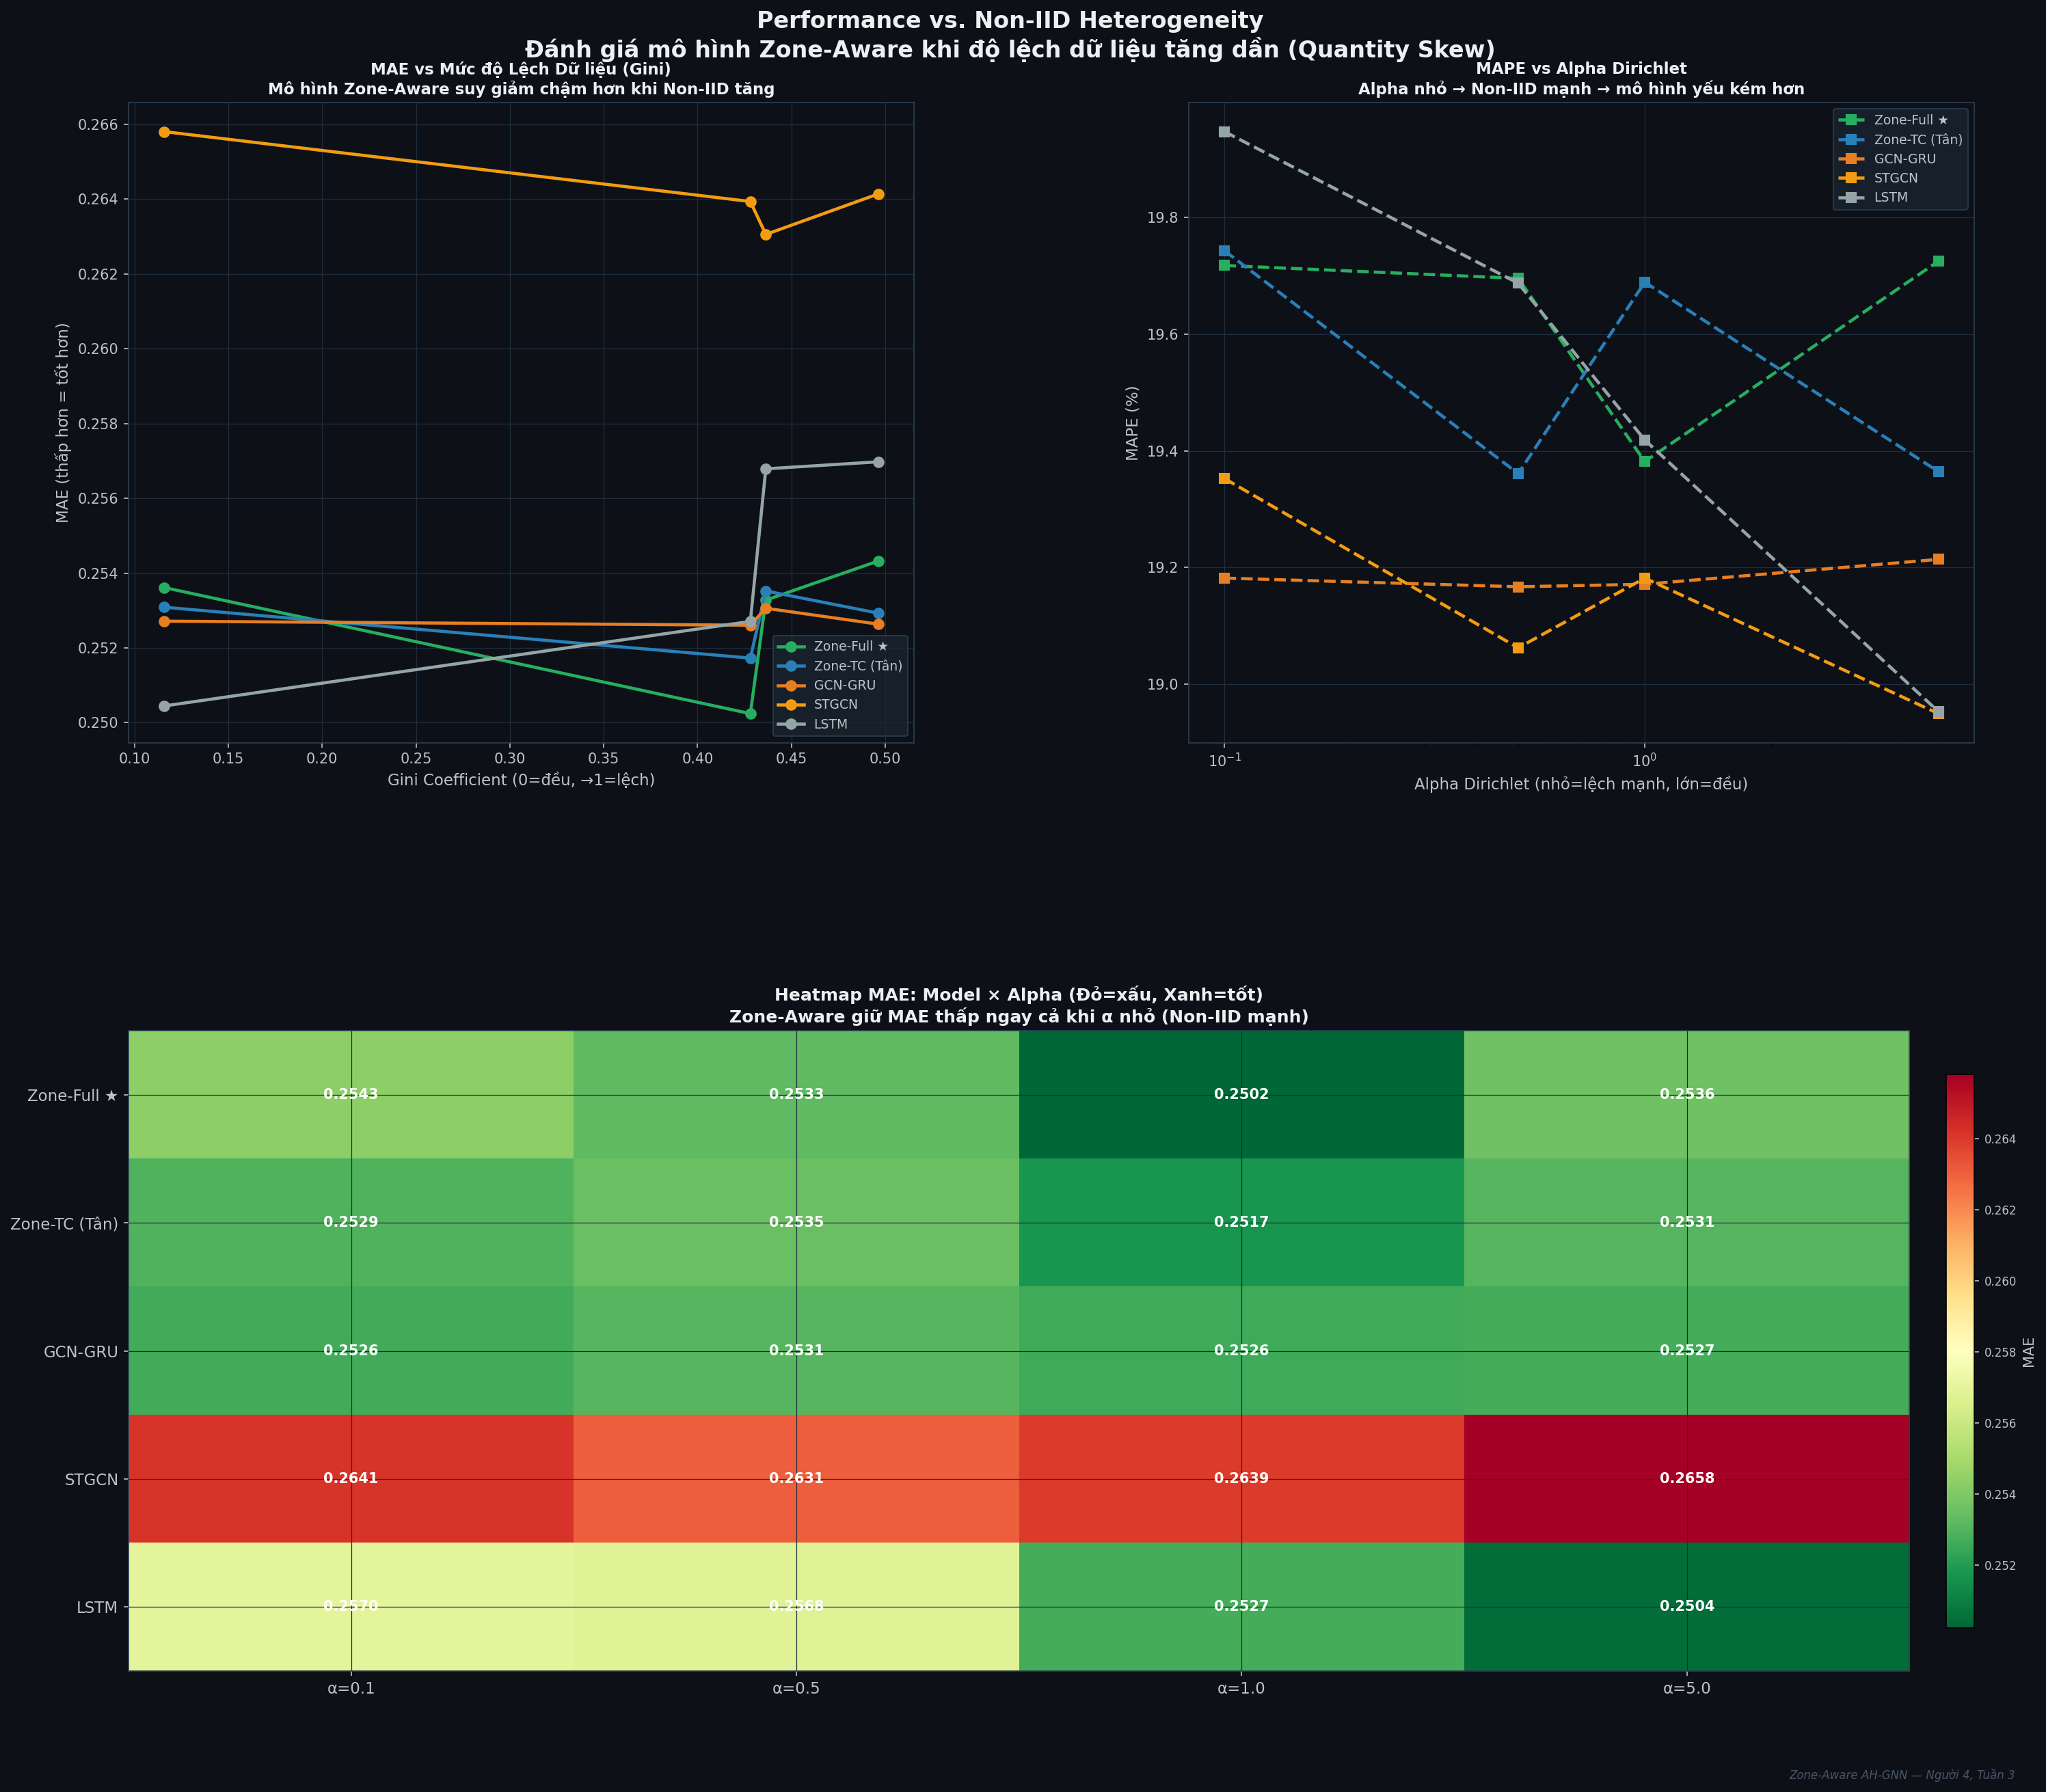
\includegraphics[width=0.98\textwidth]{../data/results/non_iid_performance.png}
        \caption{Hiệu suất mô hình theo mức độ Non-IID (Zone-Aware giữ ổn định tốt nhất)}
        \label{fig:non_iid}
    \end{figure}

\end{document}
